\documentclass[12pt]{article}

\usepackage[utf8]{inputenc}
\usepackage[russian]{babel}

\usepackage{amssymb}
\usepackage{amsmath}
\usepackage{amscd}
\usepackage{amsthm}
\usepackage{xcolor}

\usepackage{indentfirst}

%\usepackage{marginnote} % this is used for notes on the right margin --- \marginnote{\footnotesize txt}

\usepackage{mathtools} % for mathclap command

%\usepackage[normalem]{ulem} % for crossing text out - \sout

% Redefining \def is impossible. I tried, but it is impossible.
%\let\def_prev\def

%%%%%%%%%%%%%%%%%%%%%%%%%%%%%%%%%%%%%%%%%%%%%%%
%           MATH OPERATORS SPACING            %
%%%%%%%%%%%%%%%%%%%%%%%%%%%%%%%%%%%%%%%%%%%%%%%

\let\existstemp\exists
\let\foralltemp\forall
\renewcommand{\exists}{\: \existstemp \:}
\newcommand{\existsonly}{\: \existstemp ! \:}
\renewcommand{\forall}{\: \foralltemp \:}

%%%%%%%%%%%%%%%%%%%%%%%%%%%%%%%%%%%%%%%%%%%%%%%
%            COMMAND SHORTHANDS               %
%%%%%%%%%%%%%%%%%%%%%%%%%%%%%%%%%%%%%%%%%%%%%%%

\newcommand{\example}{{\itshape Пример. }}
\newcommand{\equals}{\Leftrightarrow}
\newcommand{\exc}{{\bfseries Упражнение. }}
\newcommand{\norm}[1]{\left\| #1 \right\|}
\newcommand{\scal}[2]{\left\langle #1, #2 \right\rangle}
\newcommand{\angular}[1]{\langle #1 \rangle}

\newcommand{\Sum}[2]{\underset{#1}{\overset{#2}{\sum}}}
\newcommand{\Int}[2]{\underset{#1}{\overset{#2}{\int}}}
\newcommand{\Ker}{\text{Ker}}

% Physicists' variant of dot product
\newcommand{\pscal}[2]{\, \langle #1 | #2 \rangle \,}
\newcommand{\bra}[1]{\, \langle #1 |}
\newcommand{\ket}[1]{| #1 \rangle \,}

\renewcommand{\leq}{\leqslant}
\renewcommand{\geq}{\geqslant}

%%%%%%%%%%%%%%%%%%%%%%%%%%%%%%%%%%%%%%%%%%%%%%%
%         THEOREM DEFINITION LINES            %
%%%%%%%%%%%%%%%%%%%%%%%%%%%%%%%%%%%%%%%%%%%%%%%

\newtheorem{lem}{Лемма}[section]
\newtheorem{note}{Замечание}[section]
\newtheorem{defi}{Определение}[section]
\newtheorem{theorem}{Теорема}[section]
\newtheorem{state}{Утверждение}[section] % statement

%%%%%%%%%%%%%%%%%%%%%%%%%%%%%%%%%%%%%%%%%%%%%%%
%             GRAPHICS INCLUSION              %
%%%%%%%%%%%%%%%%%%%%%%%%%%%%%%%%%%%%%%%%%%%%%%%

\usepackage{graphicx}

\graphicspath{{./Graphics/}}

%%%%%%%%%%%%%%%%%%%%%%%%%%%%%%%%%%%%%%%%%%%%%%%
%               DRAFT TEMPLATES               %
%%%%%%%%%%%%%%%%%%%%%%%%%%%%%%%%%%%%%%%%%%%%%%%

%\usepackage{marginnotes}
\newcommand{\todo}[1]{\marginpar{\color{red} \tiny #1}}

\begin{document}
	Продолжим рассмотрение полиномов Чебышёва:
	
	$$ T_n(x) = cos(n \cdot arccos(x)) $$
	$$ T_n' = n \cdot sin(n \cdot arcos(x)) \frac{1}{\sqrt{1-x^2}} $$
	$$ T_n'' = -n^2 \cdot cos(n \cdot arccos(x)) \cdot \frac{1}{1-x^2} + n \cdot sin(n \cdot arccos(x)) \frac{x}{(1-x^2)^{\frac{3}{2}}} $$
	
	Попробуем получить дифференциальное уравнение для многочленов Чебышёва. Домножая $T_n''$, увидим, что
	$$ (1-x^2) T_n'' = -n^2 T_n + x T_n' $$
	Что лёгким движением слагаемых превращается в дифференциальное уравнение:
	\begin{equation} \label{eq:Tndiffeq}
		(1-x^2) T_n'' - x T_n' + n^2 T_n = 0
	\end{equation}
	
	При помощи данного уравнения представляется возможным проверить ортогональность полиномов Чебышёва. Запишем \eqref{eq:Tndiffeq}
	отдельно для $T_n$ и $T_m$, домножив эти уравнения на $T_m$ и $T_n$ соответственно.
	
	$$ T_m \cdot ( (1-x^2)T_n'' +  x T_n' + n^2 T_n) = 0 $$
	$$ T_n \cdot ( (1-x^2)T_m'' +  x T_m' + m^2 T_m) = 0 $$
	
	Вычитая первое из второго, получаем 
	$$ (1-x^2)(T_n'' T_m - T_m'' T_n) - x(T_n' T_m - T_m' T_n) + T_n T_m (n^2 - m^2) = 0 $$
	
	Наибольший интерес для нас представляет третье слагаемое: домножив его на весовую функцию для полиномов Чебышёва 
	$h(x) = \frac{1}{\sqrt{1-x^2}}$ мы получим, с точностью до константы, подынтегральное выражение для скалярное произведения
	в рассматриваемом пространстве.
	
	$$ \int_{-1}^1 \sqrt{1-x^2} (T_n'' T_m - T_m'' T_n + \underline{T_n'T_m' - T_n'T_m'}) dx \: - $$
	$$ \int_{-1}^1 \frac{x}{\sqrt{1-x^2}} (T_n' T_m - T_m' T_n) dx +
	   \int_{-1}^1 T_n T_m \frac{n^2 - m^2}{\sqrt{1-x^2}} dx = 0 $$

	Выражение, подчеркнутое в уравнении тождественно равняется нулю; оно добавлено, руководствуясь соображениями, которые
	станут ясны из дальнейших вычислений. Возьмем второй интеграл по частям.
	$$
		\int_{-1}^1 \frac{x}{\sqrt{1-x^2}} (T_n' T_m - T_m' T_n) dx =
		\begin{tabular}{| l}
			$u = T_n' T_m - T_m' T_n$ \\
			$dv = \frac{x dx}{\sqrt{1-x^2}}$
		\end{tabular} = 
	$$
	$$
		=
		\begin{tabular}{| l}
			$du = T_n'' T_m' + T_n' T_m' - T_n' T_m' - T_n' T_m'' dx$ \\
			$v = \sqrt{1-x^2}$
		\end{tabular}
		=
	$$
	$$
		= \underbrace{u \cdot \sqrt{1-x^2} \: |_{-1}^1}_{\mathclap{\text{Равно нулю}}} - 
		\underbrace{\int v \cdot du}_{\mathclap{\qquad \text{Равно первому слагаемому}}}
	$$
	
	Отсюда, исходное равенство преобразуется в
	$$(n^2 - m^2) \int_{-1}^{1} \frac{T_n T_m}{1-x^2} = 0$$
	
	Таким образом, доказывается ортогональность полиномов Чебышёва: $\scal{T_n}{T_m} = 0$ при $n \neq m$.
	
	Покажем, что дифференциальное уравнение \eqref{eq:Tndiffeq} имеет многочлены в виде корней. Для этого, будем искать
	решение в виде бесконечного степенного ряда: 
	\begin{equation} \label{eq:Tnseries}
		T_n(x) = \sum_{k=0}^{\infty} a_k x^2
	\end{equation}
	Рассмотрим, какие будут возникать коэффициенты при различных степенях x: \\
	\begin{tabular}{l r}
		$[1]$ & $ 2a_2 + n^2 a_0 = 0 $ \\
		$[x]$ & $ 6a_3 - a_1 + n^2a_1 = 0 $ \\
		\dots \\
		$[x^k]$ & $ (k+2)(k+1) a_{k+2} - k(k-1) a_k + n^2 a_k = 0 $
	\end{tabular} \\
	Здесь несложно увидеть следующее соотношение:
	$$ a_{k+2} = \frac{(n^2 - k^2) a_k}{(k+1)(k+2)}$$
	
	В частности, из этого соотношения следует, что достаточно знать $a_0$ и $a_1$ для нахождения всех коэффициентов ряда.
	Используя эту формулу, посмотрим, когда же в решении \eqref{eq:Tndiffeq} появляются полиномы. Для этого необходимо, 
	чтобы ряд \eqref{eq:Tnseries} имел конечное число слагаемых. То есть, что равносильно при выведенном соотношении, 
	после некоторого $n$, $a_k$ становятся равны нулю. Возможно два варианта:
	\begin{enumerate}
		\item $n$ - чётное. \\
		Если при данном условии $a_1 \neq 0$, то коэффициенты $a_{2k+1}$ не равны нулю при любых k. Таким образом, налагаем
		условие $a_1 = 0$.
		\item $n$ - нечётное \\
		Аналогично предыдущему случаю, но налагается условие $a_0 = 0$.
	\end{enumerate}
	
	\subsection{Функции Хаара}
	
	Также, для полноты представления ортогональных систем, ознакомимся с функциями Хаара. В разных книгах данный термин
	может иметь разные значения. Мы обозначим функции Хаара таким образом: \\
	Рассмотрим последовательность $h_0, h_1, \dots, h_n, \dots$ в пространстве $\mathbb{L}_1(0, 1)$
	
	\begin{figure}[H]
		\begin{subfigure}[c]{0.5\textwidth}
		\vspace{-40pt}
		\begin{eqnarray*}
			h_0& =& 1 \\		
			h_1& =& 
			\begin{cases}
				1, & x < \frac{1}{2} \\
				-1, & x \geq \frac{1}{2}
			\end{cases} \\		
			h_2& =& 
			\begin{cases}
				\sqrt{2}, & x < \frac{1}{4} \\
				-\sqrt{2}, & x \geq \frac{1}{4} \\
				0, & x \geq \frac{1}{2}
			\end{cases}
		\end{eqnarray*}
		\end{subfigure}
		~
		\begin{subfigure}[c]{0.5\textwidth}
			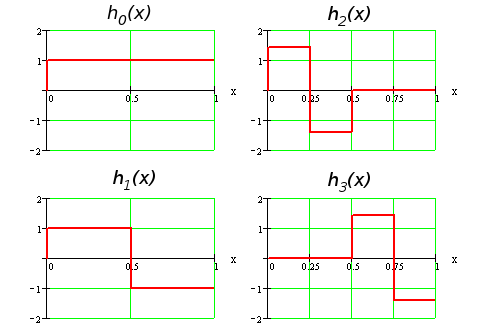
\includegraphics[width=0.95\textwidth]{../Graphics/Lectures-5-Haar_functions.png}
			\caption{Графики некоторых функций Хаара.}
		\end{subfigure}
	\end{figure}
	
	И так далее, образуя последовательность ортогональных ступенчатых функций. Любая функция, являющеаяся ступенчатой, может
	быть задана через линейную последовательность функций $h_0, \dots, h_n, \dots$.
	
	\section{Линейные операторы}
	
	Прежде чем начать изучение линейных операторов, стоит предупредить, что буквы, используемые нами для обозначения некоторых
	классических операторов, могут не являться общепринятыми и отличаться от принятых в различной литературе по данному предмету.
	
	\begin{defi}
		Отображение $A$ из $M$ в $L$ назовём \textbf{линейным оператором}, если область определения оператора
		$D(A) \subset M$ и выполнены следующие условия:
		\begin{enumerate}
			\item $A(x + y) = Ax + Ay$
			\item $A(\alpha x) = \alpha A x$ 
		\end{enumerate}
		Обозначают $A : M \rightarrow L$.
	\end{defi}
	
	Впрочем, определение линейного оператора уже рассматривалось в курсе линейной алгебры. Для применения линейных операторов в
	нашем курсе, будем предполагать, что $M$ и $L$ --- нормированные пространства. А если есть норма $\Rightarrow$ есть расстояние
	$\Rightarrow$ может быть определена непрерывность. Если $A$ непрерывно в $h_0$, пишут:
	
	$$ \forall \varepsilon > 0 \exists \delta > 0 : \forall h \: \norm{h - h_0} < \delta \Rightarrow \norm{Ah  Ah_0} 
	= \norm{A(h-h_0)} < \varepsilon $$
	Нетрудно видеть, что из непрерывности в точке следует непрерывность в нуле --- для этого нужно взять $h := h + h_0$. 
	Так же можно сделать для любой точки множества. Значит, $A$ непрерывна на всём множестве. Тогда, исходя из данного
	определения, получаем равномерную непрерывность для $A$.
	
	Приведём некоторые примеры линейных операторов:
	\begin{itemize}
		\item Тождественный оператор
		\item Нулевой оператор
		\item Оператор проектирования на замкнутое подпространство гильбертова пространства.
		\item $f(t) \rightarrow t \cdot f(t)$ в пространстве $\mathbb{L}_2 (0,1) \rightarrow \mathbb{L}_2 (0,1)$
		\item Оператор дифференцирования: $\text{\emph{D}}: \mathbb{L}_2 (0,1) \rightarrow \mathbb{L}_2 (0,1)$. Отметим также, что
		область определения этого оператора $D(\text{\emph{D}}) \neq \mathbb{L}_2 (0,1)$
		\item $f(x) \rightarrow \int_0^x f(t) dt$.
	\end{itemize}
	
	Для существования обратного оператора $A^{-1}$ нужно:
	\begin{enumerate}
		\item $A$ - инъективно.
		\item $D(A^{-1}) = $ образ прямого отображения
	\end{enumerate}
	В наших обозначениях, обратный оператор всегда определяет обратное отображение.

	\subsection{Ограниченный линейный оператор}	
	
	\begin{defi}
		Множество ограничено, если существет шар с центром в точке $O$, в котором содержится все множество.
	\end{defi}
	\begin{defi}
		Множество $M$ \textbf{ограничено}, если существет шар $B_r(a)$, в котором содержится все множество:
		$$ \exists a \in X \; \exists (r > 0) \; \forall x \in X (x \in M \Rightarrow \rho(a, x) < r) $$
	\end{defi}
	\begin{defi}
		Оператор $A: M \Rightarrow L$ называется \textbf{ограниченным}, если он переводит ограниченное множество
		в ограниченное.
	\end{defi}
	
	\begin{state}
		Линейный оператор ограничен $\equals$ он непрерывен.
	\end{state}
	\begin{proof}
		\textbf{Необходимость}. Если $A$ --- непрерывный оператор, то 
		$ \exists \delta : \norm{h} < \delta \Rightarrow \norm{Ah} < 1 $,
		откуда следует, что $\norm{h} < R$. 
		
		Рассмотрим вектор $x = \frac{\delta h}{R}$. В указанных условиях
		$\norm{x} < \frac{\delta}{R}$, откуда следует $\norm{Ax} < 1$ и, из линейности оператора и свойств нормы:

		$$\frac{\delta}{R} \cdot \norm {Ah} < 1$$
		
		Это означает, что отображение $A$ переводит все значения в шар радиуса $\frac{R}{\delta}$, значит
		$A$ --- ограниченный оператор. \\
		
		\textbf{Достаточность}. Аналогично доказательству необходимости. Если $A$ --- ограниченный оператор,
		то при $\norm{h} \leq 1$ получается $\norm{Ah} \leq R$. Возьмём шар радиуса $\frac{\varepsilon}{R}$
		и действуем так же, как в предыдущем доказательстве.
	\end{proof}
	
	\subsection{Норма линейного оператора}
	
	\begin{defi}
		\textbf{Нормой линейного оператора} $A$ называется выражение вида 
		$$\norm{A} \overset{df}{=} \underset{x \neq 0}{sup} \frac{\norm{Ax}}{\norm{x}}$$
	\end{defi}
	
	\begin{state}
		Линейный оператор ограничен $\equals$ его норма конечна.
	\end{state}
	\begin{proof}
		Распишем норму линейного оператора:
		$$
			\norm{A} \overset{df}{=} \underset{x \neq 0}{sup} \frac{\norm{Ax}}{\norm{x}} = 
			\underset{x \neq 0}{sup} \norm{A \frac{x}{\norm{x}}} =
			\underset{\norm{y} = 1}{sup} \norm{Ay} \leq
		$$
		$$
			\leq
			\underset{0 \leq \norm{y} \leq 1}{sup} \norm{Ay} \leq
			\underset{0 \leq \norm{y} \leq 1}{sup} \frac{\norm{Ay}}{\norm{y}} \leq
			\underset{y \neq 0}{sup} \frac{\norm{Ay}}{\norm{y}} =
			\norm{A}
		$$
		Так как все неравенства, приведенные здесь, были направлены в одну сторону,
		они обратятся в равенства. При этом, последнее равенство гарантирует, что
		оператор $A$ переведёт вектор $\norm{h} \leq r$ в замкнутый шар радиуса $\norm{A} \cdot r$.
		С другой стороны, при ограниченности оператора, его норма будет конечна, по приведённым
		выше равенствам.
	\end{proof}
	
	Сделаем также ещё одно замечание, исходящее из определения:
	$$ \frac{\norm{Ax}}{\norm{x}} \leq \norm{A} $$
	$$ \norm{Ax} \leq \norm{A} \cdot \norm{x} $$
	
	Мы в очередной раз что-то назвали нормой. Но {\color{gray}гуманно} верно ли это?
	
	\exc Для нормы линейного оператора выполнены все аксиомы нормы.
	% TODO: потом хотелось бы написать здесь доказательство и переписать это как "Утверждение".
	
	Также, остается упражнение по доказательству еще одного полезного свойства:
	
	\exc Доказать выполнение равенства $\norm{A} - \norm{B} \leq \norm{A-B}$.
	
	\begin{state}
		$$\norm{Ax} \leq k \norm{x} \Rightarrow \norm{A} \leq k$$
	\end{state}
	
	\begin{state}
		Для нормы композиции линейных операторов верно неравенство 
		$$\norm{A\cdot B} \leq \norm{A} \cdot \norm{B}$$
	\end{state}
	\begin{proof}
		$$ \norm{(AB)x} = \norm{A(Bx)} \leq \norm{A} \cdot \norm{Bx} \leq \norm{x} \cdot \norm{A} \cdot \norm{B} $$
		Отсюда 
		$$ \norm{AB} \leq \norm{A} \cdot \norm{B} $$
		что и требовалось доказать. \\
	\end{proof}
	
	\subsection{Оператор Гильберта-Шмидта}
	Рассмотрим пространства $\mathbb{L}_2(\mathbb{R}^n)$ и $\mathbb{L}_2(\mathbb{R}^k)$, а также функцию
	$$ k(x,y) \in \mathbb{L}_2(\mathbb{R}^{n+k}), x \in \mathbb{R}^n, y \in \mathbb{R}^k$$
	
	\begin{defi}
		\textbf{Оператором Гильберта-Шмидта} назовём оператор:
		$$ (Af)(t) \overset{df}{=} \underset{\mathbb{R}^k}{\int} k(t,y) f(y) dy $$
	\end{defi}
	
	Покажем, что функция $(Af)(t)$ определена почти для всех $t$. Пользуясь определением скалярного произведения в $\mathbb{L}_2$, 
	видим, что $\norm{(Af)(t)}^2 = (\scal{f}{k})^2 \leq \norm{f}^2 \cdot \underset{\text{на }\mathbb{R}^k}{\norm{k}^2}$
	
	$$ \norm{(Af)(t)}^2 \leq \underset{\mathbb{R}^k}{\int} |f(y)|^2 dy \cdot \underset{\mathbb{R}^k}{\int} |k(t,y)|^2 dy $$
	
	Проинтегрируем обе части выражения по множеству $\mathbb{R}^n$:
	
	$$ \Int{\mathbb{R}^n}{} \norm{(Af)(t)}^2 \, dt \leq \underset{\mathbb{R}^k}{\int} |f(y)|^2 \, dy 
	   \cdot \Int{\mathbb{R}^n}{} \Int{\mathbb{R}^k}{} |k(t,y)|^2 \, dt \, dy $$
	
	$k(t,y)$ почти всюду определена в $\mathbb{R}^k$, интегрируема
	в $\mathbb{R}^k$ по условию. Значит, по теореме Фубини можем переставить пределы интегрирования 
	и перейти к норме на $\mathbb{R}^n$.
	
	$$ \Int{\mathbb{R}^n}{} \norm{(Af)(t)}^2 \, dt \leq \norm{f}^2_{\mathbb{L}_2} \cdot \norm{k}^2_{\mathbb{L}_2} $$
\end{document}